
\documentclass[a4paper,12pt]{article} % тип документа


% Русский язык
\usepackage[T2A]{fontenc} % кодировка
\usepackage[utf8]{inputenc} % кодировка исходного текста
\usepackage[russian,english]{babel} % локализация и переносы
\usepackage{graphicx}
\graphicspath{{pictures/}}
\DeclareGraphicsExtensions{.pdf,.png,.jpg}


% Математика
\usepackage{amsmath,amsfonts,amssymb,amsthm,mathtools}


\usepackage{wasysym}

%Заговолок
\author{Талашкевич Даниил Александрович}

\title{Лабораторная работа 1.1.4}

\date{\today}

\begin{document}

\maketitle
\thispagestyle{empty}

\newpage
\setcounter{page}{1}


{\bf 1. Аннотация}

Применение методов обработки экспериментальных данных для изучения статистических закономерностей при измерении интенсивности радиоционного фона.

{\bf 2. Используемое оборудование}

счётчик Гейгера-Мюллера (СТС-6), блок питания, компьютер с интерфейсом связи со счетчиком.

{\bf 3. Теоретические сведения}

В лабораторной работе изучаются космические лучи-потоки частиц, заполняющие межзвездное пространство и постоянно бомбардирующие Землю. Основной величиной, характеризующей количество частиц в космических лучах является интенсивность $I$ - число частиц, подающих в единицу времени на единичную площадку, перпендикулярную к направлению наблюдения, отнесенное к $ERROR$. В случае изотропного излучения интенсивность $I$ связана с плотностью потока формулой $F = \pi I$, обе величины -- флуктуирующие.

Для измерения итенсивности лучей мы будем использовать счетчик Гейгера=Мюллера. Частицы космических лучей пролетают через газ, которым наполнен счетчик, ионизируя его и выюивая электроны из его стенок. На электроды счетчика падается напряжение $400B$, из-за чего электроны ускоряются и выюивают из молекул газа вторичные электроны, затем они снова ускоряются и ионизируют молекулы газа -- в результате образуется электронная лавина, и через счетчик резко увеличивается ток.

Экспериментальная схема показана на рисунке.


При возникновении тока через счетчик конденсатор $C_1$ использует свой заряд, передавая его счетчику(для тока). Разряд в счетчике прекращается, когда ток достаточно мал, чтобы разность потенциалов между электролами оказалась меньше потенциала ионизации молекул газа.Далее конденсатор $C_1$ заряжается за время релаксации $\tau = kRC_1$, где $k$ -- значение порядка единицы, при чем в течении этого времени счетчик не может регистрировать частицы -- мертвое время. Таким образом, значение $C_1$ должно быть ни большим, ни малым, а $R$ малым(для уменьшения мертвого времени), но таким, чтобы разряд не был слишком долгом, то есть чтобы коденсатор $C_1$ не успевал заряжаться во время разряда на счетчике (обычно $R \approx k \textbf{МОм}$, где $K \sim 1$). Конденсатор $C_1$ нужен для того, чтобы не пропускать постоянное напряжение блока питания к компьютеру. Собранная схема нужна для проведения эксперимента, описанного в ходе работы.

{\bf Ход работы}

1) Включаем счетчик Гейгера-Мюллера, затем компьютеря, предварительно собрав электрическую схему, полностью описанную выше. Запускаем программу $STAT$ для начала проведения основного эксперимента.

Длительность эксперимента: $4000\ c$.

2) Измеряем плотность потока космического излучения за $20\ с$: составляем таблицу срабатываний счетч ка Гейгера на основе снятых данных с компьютера {\bf (табл.1)}.

3) Запишем в таблицу измеренные данные для построения гистограммы распределения числа срабатываний счетчика за 10 секунд {\bf (табл.2)}.

4) С помощью таблицы 1 переведем полученные значения в таблицу количества срабатываний счетчика за 40 секунд {\bf (табл.3)}.

5) Запишем в таблицу измеренные данные для построения гистограммы распределения числа срабатываний счетчика за 40 секунд {\bf (табл. 4)}.

6) Построим гистограмму по полученным данных так, чтоюы их масштабы были примерно одинаковы {\bf (гист.1)}.

7) Найдем среднее значение числа срабатывания счетчика:

{\bf a)} $t = 10\ \textbf{c}$.

$\overline{n_1} = \frac{1}{N_1}\sum\limits_{i = 1}^{N_1}n_i = \frac{5346}{400} \approx 13.37$.

\hspace{1mm}

{\bf б)} $t = 40\ \textbf{c}$.

$\overline{n_2} = \frac{1}{N_2}\sum\limits_{i = 1}^{N_2}n_i = \frac{5339}{100} \approx 53,39$.

Таблица 1. Число срабатывания счетчика за $20\ c$.

\begin{tabular}{ | c | c | c | c | c | c | c | c | c | c | c |}
\hline
$\textbf{№ опыта}$ & $1$ & $2$ & $3$ & $4$ & $5$ & $6$ & $7$ & $8$ & $9$ & $10$\\ \hline
$0$ & $24$ & $31$ & $29$ & $17$ & $28$ & $27$ & $18$ & $22$ & $32$ & $34$ \\ \hline
$10$ & $28$ & $14$ & $31$ & $33$ & $30$ & $22$ & $33$ & $25$ & $28$ & $29$\\ \hline
$20$ & $30$ & $34$ & $27$ & $27$ & $21$ & $24$ & $28$ & $33$ & $25$ & $24$\\\hline
$30$ & $31$ & $31$ & $30$ & $25$ & $30$ & $23$ & $28$ & $21$ & $27$ & $22$\\ \hline
$40$ & $31$ & $28$ & $25$ & $28$ & $25$ & $19$ & $30$ & $22$ & $17$ & $21$\\ \hline
$50$ & $24$ & $28$ & $21$ & $28$ & $27$ & $28$ & $26$ & $26$ & $27$ & $20$\\ \hline
$60$ & $21$ & $25$ & $24$ & $15$ & $30$ & $26$ & $29$ & $29$ & $36$ & $22$\\ \hline
$70$ & $26$ & $24$ & $31$ & $30$ & $22$ & $29$ & $22$ & $30$ & $33$ & $21$\\ \hline
$80$ & $23$ & $19$ & $35$ & $20$ & $25$ & $25$ & $38$ & $21$ & $27$ & $23$\\ \hline
$90$ & $30$ & $37$ & $30$ & $27$ & $25$ & $25$ & $29$ & $28$ & $35$ & $29$\\ \hline
$100$ & $27$ & $31$ & $30$ & $24$ & $27$ & $27$ & $23$ & $22$ & $21$ & $31$\\ \hline
$110$ & $32$ & $40$ & $22$ & $24$ & $39$ & $24$ & $32$ & $24$ & $31$ & $19$\\ \hline
$120$ & $24$ & $25$ & $20$ & $21$ & $30$ & $28$ & $31$ & $25$ & $28$ & $29$\\ \hline
$130$ & $31$ & $30$ & $33$ & $28$ & $27$ & $23$ & $28$ & $28$ & $35$ & $26$\\ \hline
$140$ & $22$ & $29$ & $29$ & $29$ & $27$ & $25$ & $26$ & $28$ & $23$ & $23$\\ \hline
$150$ & $30$ & $31$ & $29$ & $25$ & $30$ & $23$ & $33$ & $23$ & $30$ & $26$\\ \hline
$160$ & $21$ & $20$ & $24$ & $17$ & $27$ & $25$ & $33$ & $20$ & $31$ & $26$\\ \hline
$170$ & $30$ & $26$ & $28$ & $29$ & $28$ & $32$ & $30$ & $30$ & $23$ & $18$\\ \hline
$180$ & $24$ & $30$ & $27$ & $25$ & $27$ & $32$ & $24$ & $32$ & $17$ & $30$\\ \hline
$190$ & $22$ & $40$ & $21$ & $19$ & $22$ & $27$ & $26$ & $24$ & $24$ & $31$\\
\hline 
\end{tabular}\\

Таблица 2. Данные для гистограммы (кол-во срабатываний за $10\ c$).

\begin{tabular}{ | c | c | c |}
\hline
$\textbf{число импульсов}$ & $\textbf{число случаев}$ & $\textbf{доля случаев}$\\ \hline
$0$ & $0$ & $0$\\ \hline
$1$ & $0$ & $0$\\ \hline
$2$ & $0$ & $0$\\ \hline
$3$ & $0$ & $0$\\ \hline
$4$ & $0$ & $0$\\ \hline
$5$ & $0$ & $0$\\ \hline
$6$ & $7$ & $0.0175$\\ \hline
$7$ & $8$ & $0.02$\\ \hline
$8$ & $13$ & $0.0325$\\ \hline
$9$ & $14$ & $0.035$\\ \hline
$10$ & $26$ & $0.065$\\ \hline
$11$ & $56$ & $0.14$\\ \hline
$12$ & $45$ & $0.1125$\\ \hline
$13$ & $41$ & $0.1025$\\ \hline
$14$ & $45$ & $0.1125$\\ \hline
$15$ & $49$ & $0.1225$\\ \hline
$16$ & $35$ & $0.0875$\\ \hline
$17$ & $16$ & $0.04$\\ \hline
$18$ & $19$ & $0.0475$\\ \hline
$19$ & $10$ & $0.025$\\ \hline
$20$ & $7$ & $0.0175$\\ \hline
$21$ & $4$ & $0.01$\\ \hline
$22$ & $3$ & $0.0075$\\ \hline
$23$ & $1$ & $0.0025$\\ \hline
$24$ & $0$ & $0$\\ \hline
$25$ & $0$ & $0$\\ \hline
$26$ & $0$ & $0$\\ \hline
$27$ & $1$ & $0.0025$\\ \hline
$28$ & $0$ & $0$\\
\hline 
\end{tabular}\\

\newpage
Таблица 3. Числа срабатываний счетчика за $40\ c$.

\begin{tabular}{ | c | c | c | c | c | c | c | c | c | c | c |}
\hline
$\textbf{№ опыта}$ & $1$ & $2$ & $3$ & $4$ & $5$ & $6$ & $7$ & $8$ & $9$ & $10$\\ \hline
$0$ & $55$ & $46$ & $55$ & $40$ & $66$ & $42$ & $64$ & $52$ & $58$ & $57$\\ \hline
$10$ & $64$ & $54$ & $45$ & $61$ & $49$ & $62$ & $55$ & $53$ & $49$ & $49$ \\ \hline
$20$ & $59$ & $53$ & $44$ & $55$ & $38$ & $52$ & $49$ & $55$ & $52$ & $47$ \\ \hline
$30$ & $46$ & $39$ & $56$ & $58$ & $58$ & $50$ & $61$ & $51$ & $52$ & $54$ \\ \hline
$40$ & $42$ & $55$ & $50$ & $59$ & $50$ & $67$ & $57$ & $50$ & $57$ & $64$ \\ \hline
$50$ & $58$ & $54$ & $54$ & $45$ & $52$ & $72$ & $46$ & $63$ & $56$ & $50$ \\ \hline
$60$ & $49$ & $41$ & $58$ & $56$ & $57$ & $61$ & $61$ & $50$ & $56$ & $61$ \\ \hline
$70$ & $51$ & $58$ & $52$ & $54$ & $46$ & $61$ & $54$ & $53$ & $56$ & $56$ \\ \hline
$80$ & $41$ & $41$ & $52$ & $53$ & $57$ & $56$ & $57$ & $60$ & $60$ & $41$ \\ \hline
$90$ & $54$ & $52$ & $59$ & $56$ & $47$ & $62$ & $40$ & $49$ & $50$ & $55$ \\

\hline 
\end{tabular}\\


\newpage
Таблица 4. Данные для гистограммы (кол-во срабатываний за $40\ c$).

\begin{tabular}{ | c | c | c |}
\hline
$\textbf{число импульсов}$ & $\textbf{число случаев}$ & $\textbf{доля случаев}$\\ \hline
$38$ & $1$ & $0.01$\\ \hline
$39$ & $1$ & $0.01$\\ \hline
$40$ & $2$ & $0.02$\\ \hline
$41$ & $4$ & $0.04$\\ \hline
$42$ & $2$ & $0.02$\\ \hline
$43$ & $0$ & $0$\\ \hline
$44$ & $1$ & $0.01$\\ \hline
$45$ & $2$ & $0.02$\\ \hline
$46$ & $4$ & $0.04$\\ \hline
$47$ & $2$ & $0.02$\\ \hline
$48$ & $0$ & $0$\\ \hline
$49$ & $6$ & $0.06$\\ \hline
$50$ & $7$ & $0.07$\\ \hline
$51$ & $2$ & $0.02$\\ \hline
$52$ & $8$ & $0.08$\\ \hline
$53$ & $4$ & $0.04$\\ \hline
$54$ & $7$ & $0.07$\\ \hline
$55$ & $7$ & $0.07$\\ \hline
$56$ & $8$ & $0.08$\\ \hline
$57$ & $6$ & $0.06$\\ \hline
$58$ & $6$ & $0.06$\\ \hline
$59$ & $3$ & $0.03$\\ \hline
$60$ & $2$ & $0.02$\\ \hline
$61$ & $6$ & $0.06$\\ \hline
$62$ & $2$ & $0.02$\\ \hline
$63$ & $1$ & $0.01$\\ \hline
$64$ & $3$ & $0.03$\\ \hline
$65$ & $0$ & $0$\\ \hline
$66$ & $1$ & $0.01$\\ \hline
$67$ & $1$ & $0.01$\\ \hline
$68$ & $0$ & $0$\\ \hline
$69$ & $0$ & $0$\\ \hline
$70$ & $0$ & $0$\\ \hline
$71$ & $0$ & $0$\\ \hline
$72$ & $1$ & $0.01$\\
\hline 
\end{tabular}\\



8) Найдем среднеквадратичную ошибку отдельного измерения :


{\bf a)} $t = 10\ \textbf{c}$.

$ \sigma_1 = \sqrt{\frac{1}{N_1}\sum\limits_{i = 1}^{N_1}(n_i - \overline{n_1})^2} = \sqrt{\frac{4409}{400}} \approx 3,32$.

\hspace{1mm}

{\bf б)} $t = 40\ \textbf{c}$.

$ \sigma_2 = \sqrt{\frac{1}{N_2}\sum\limits_{i = 1}^{N_2}(n_i - \overline{n_2})^2} = \sqrt{\frac{4508}{100}}\approx  6,71$.

9) Убедимся в справедливости формулы  $\sigma_k = \sqrt{\frac{1}{N_k}\sum\limits_{i = 1}^{N_k}(n_i - \overline{n_k})^2} \approx \sqrt{\overline{n_k}}$.

{\bf a)} $t = 10\ \textbf{c}$.

$ \sigma_1^{\textbf{'}} =  3,65 \approx 1,1\cdot \sigma_1$.

\hspace{1mm} 

{\bf б)} $t = 40\ \textbf{c}$.

$ \sigma_2^{\textbf{'}} =  7,3\approx 1,09\cdot\sigma_2$.

Полученные данные примерно сходятся $ \Rightarrow $ формула справедлива.

10)Определим долю случаев, когда отклонение от среднего значения не превыщают $\sigma_1,2\sigma_1$ и сравним с теоретическими оценками.

\begin{tabular}{ | c | c | c | c | }
\hline
$\textbf{Ошибка}$ & $\textbf{Число случаев}$ & $\textbf{Доля случаев,\%}$ & $\textbf{Теор.оценка,\% }$\\ \hline
$\pm \sigma_1 = \pm 3,32$ & $270$ & $67,6$ & $0$\\ \hline
$\pm 2\sigma_1 = \pm 6,64$  & $382$ & $95,6$ & $0$\\
\hline 
\end{tabular}\\

Теоретические оценки практически совпадают с экспериментальными данными.

11) Сравним среднеквадратичные ошибки отдельных измерений для двух распределений : $\overline{n_1} = 13,37$, $\sigma_1 = 3,32$, $\overline{n_2} = 53,39$ , $\sigma_2 = 6,71$ . Легко виделть, что хотя абсолютное значение $\sigma$ во втором распределении больше, чем в первом ($ > $), относительная полуширина второго распределения меньше :

$ \frac{\sigma_1}{\overline{n_1}}\cdot 100\% = \frac{3,32}{13,37}\cdot 100\% \approx 24,8\%$, 
$\  \frac{\sigma_2}{\overline{n_2}}\cdot 100\% = \frac{6,71}{53,39}\approx 12,6 \%$.

Это так же следует из гистограммы (см. гист 1).

12) Определим стандартную ошибку величин $\overline{n_1}$ и $\overline{n_2}$ :

\[  \sigma_{\overline{n_1}} = \frac{\sigma_1}{\sqrt{N_1}} = \frac{3,32}{\sqrt{400}} \approx 0,17 \textbf{, }\ \sigma_{\overline{n_2}} = \frac{\sigma_2}{\sqrt{N_2}} = \frac{6,71}{\sqrt{100}}\approx 0,67 \ .\]

Найдем относительную ошибку :

\[ \varepsilon_{\overline{n_1}} = \frac{\sigma_{\overline{n_1}}}{\overline{n_1}}\cdot 100\% = \frac{0,17}{13,37}\cdot 100\% \approx 1,27\% \textbf{,  } \varepsilon_{\overline{n_2}} = \frac{\sigma_{\overline{n_2}}}{\overline{n_2}}\cdot 100\% = \frac{0,67}{53,39}\cdot 100\% \approx 1,25\% \ .\]

( теор. оценка $\varepsilon_{n_1}^{\textbf{'}}= \frac{100\%}{\sqrt{\overline{n_1}N_1}} \approx 1,37\%$,\hspace{1mm} $ \varepsilon_{n_2}^{\textbf{'}}= \frac{100\%}{\sqrt{\overline{n_2}N_2}} \approx 1.36\%\ . $ 

13) Строим гистограмму на основе таблице 2 и 4, причем там, чтобы данные удобно располагались на ней (см. след. страницу).

14) Окончательный результат :
\[ n_{40} = \overline{n_2} \pm \sigma_{\overline{n_2}} = 53,39 \pm 0.67 \ . \]

\[ n_{10} = \overline{n_1} \pm \sigma_{\overline{n_1}} = 13,37 \pm 0,17 \ . \]

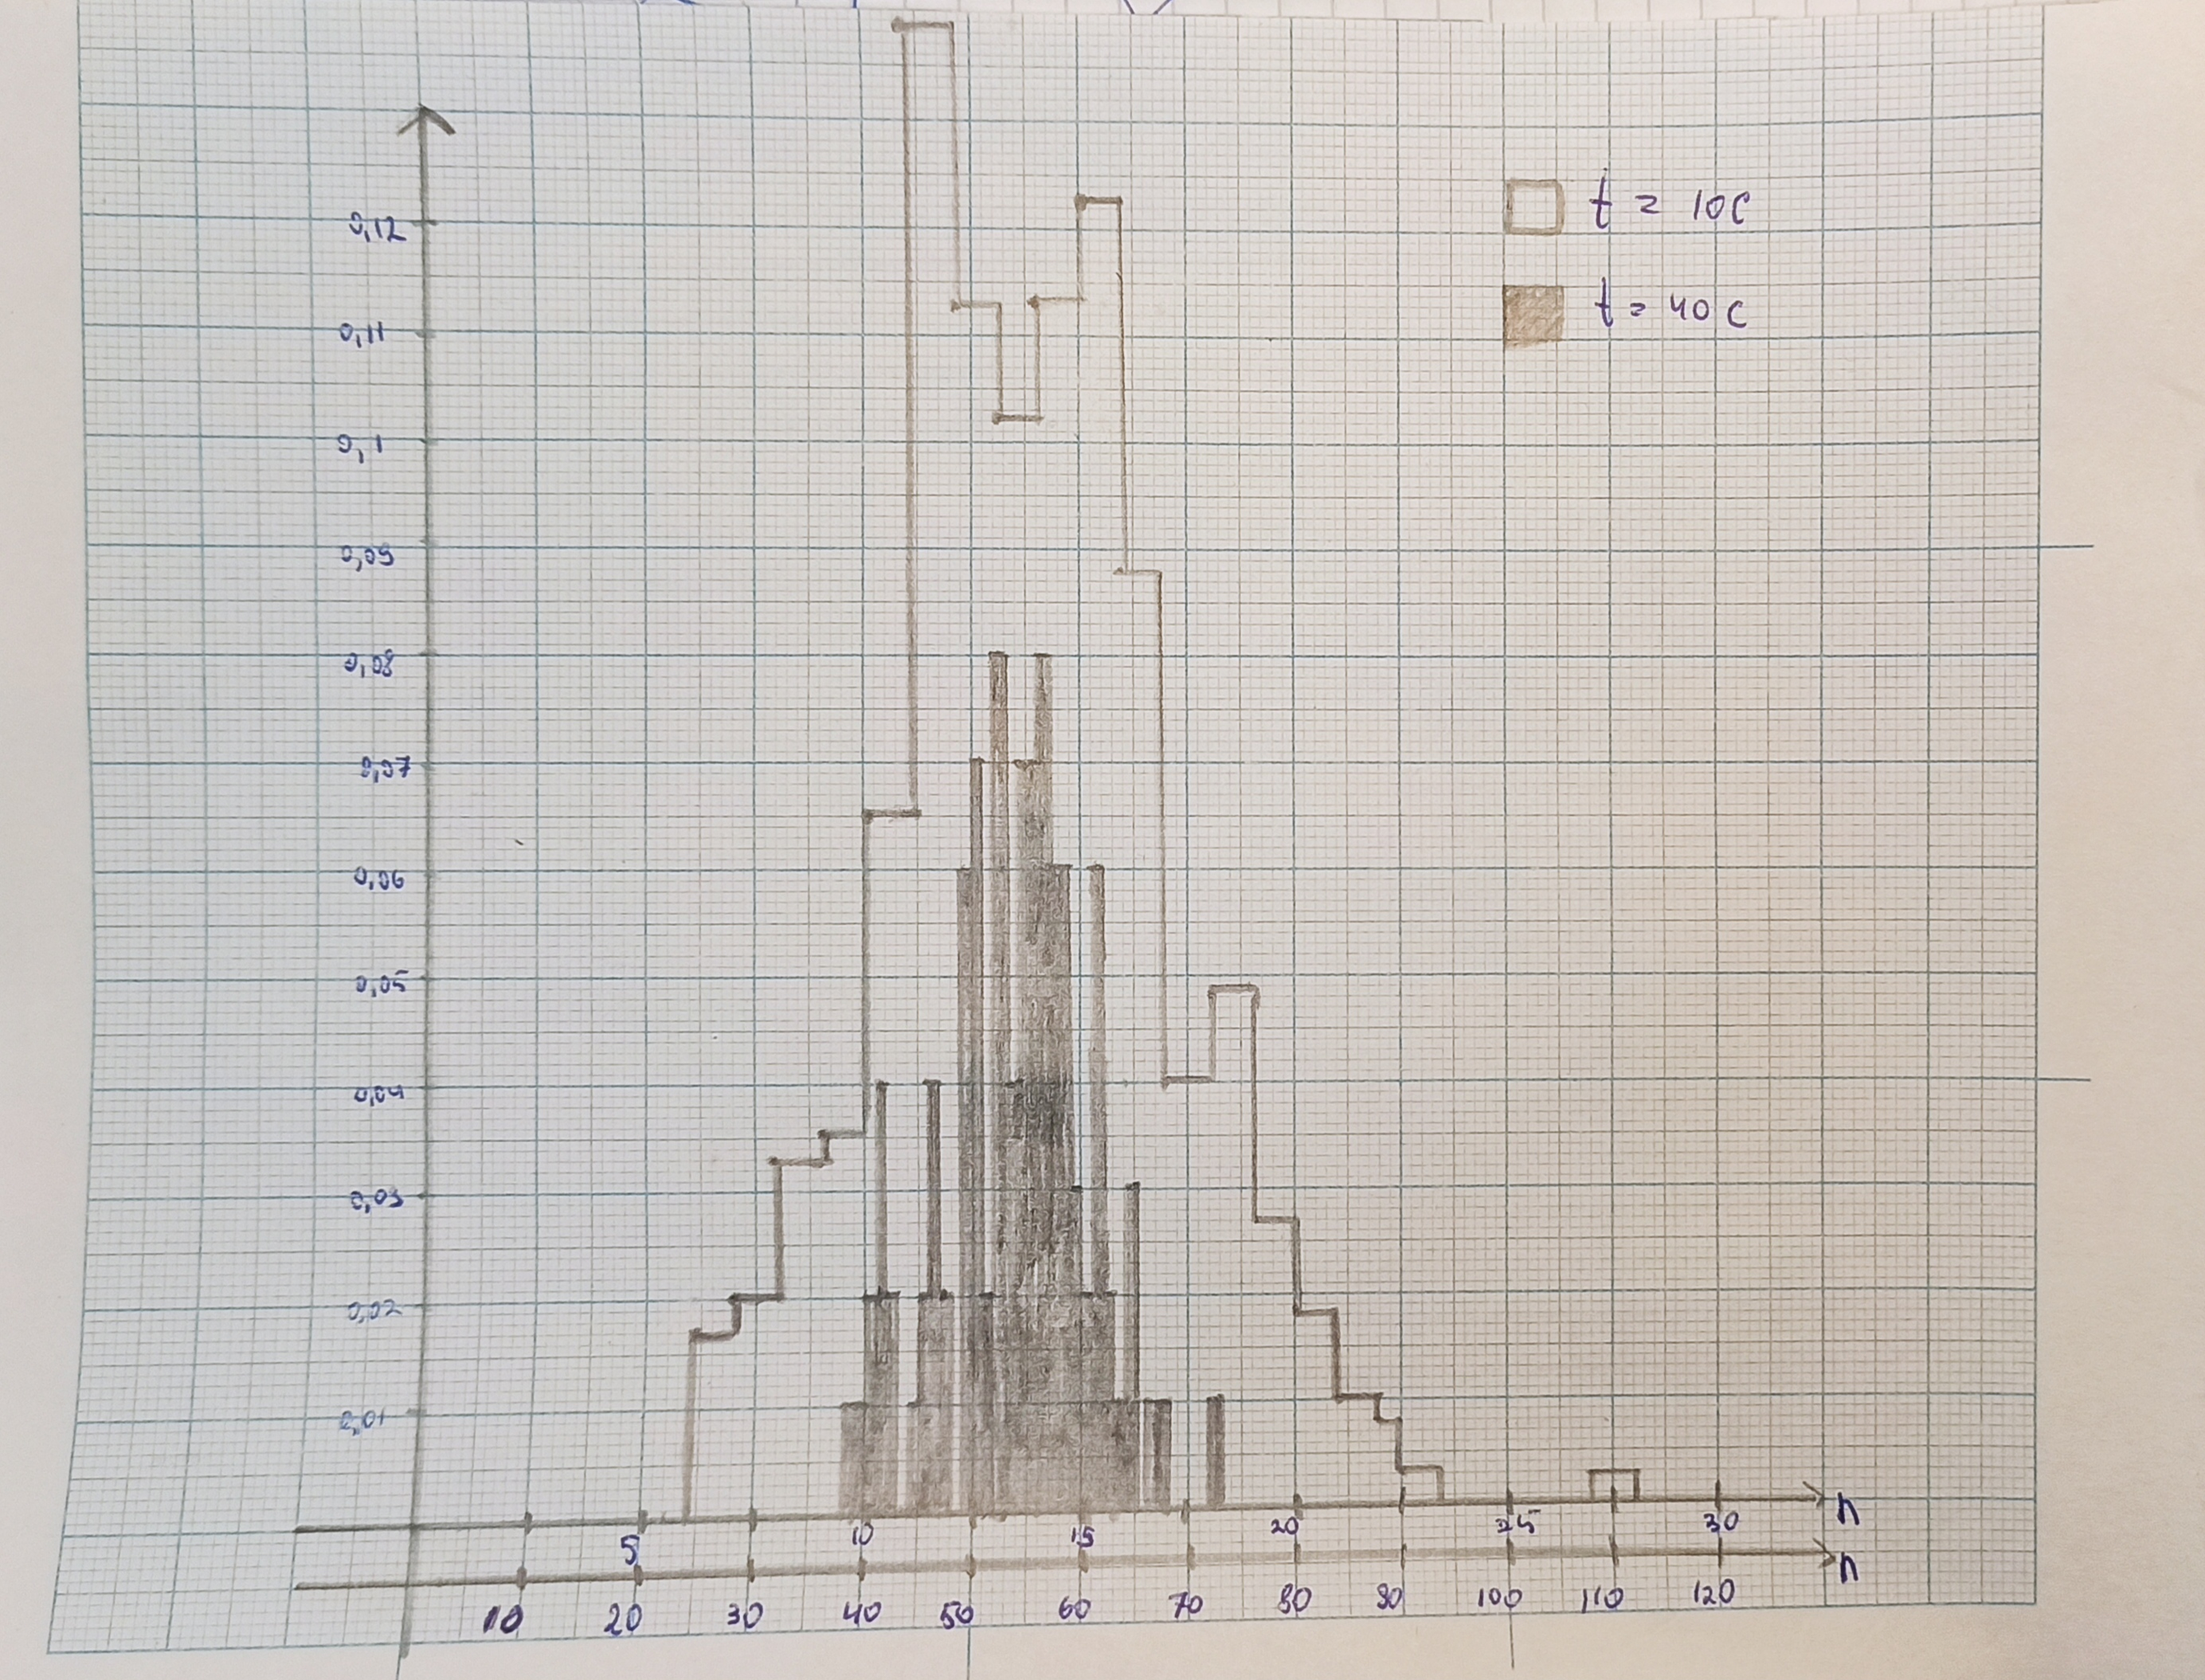
\includegraphics[width=\textwidth]{1.1.4.jpg}

Вывод : применив методы обработки экспериментальных данных мы изучали статистические закономерности при измерении интенсивности радиационного фона. Узнали, что из себя представляет и как работает счетчик Гейгера-Мюллера и экспериментально подтвердили теоретические формулы.











${\bf }$









\end{document}


